\appendix
\clearpage
\addappheadtotoc
\appendixpage


%------------------ANEXO I--------------------
\chapter{Anexo I: Documentación de la etapa de control}\label{anexo1}
\newpage

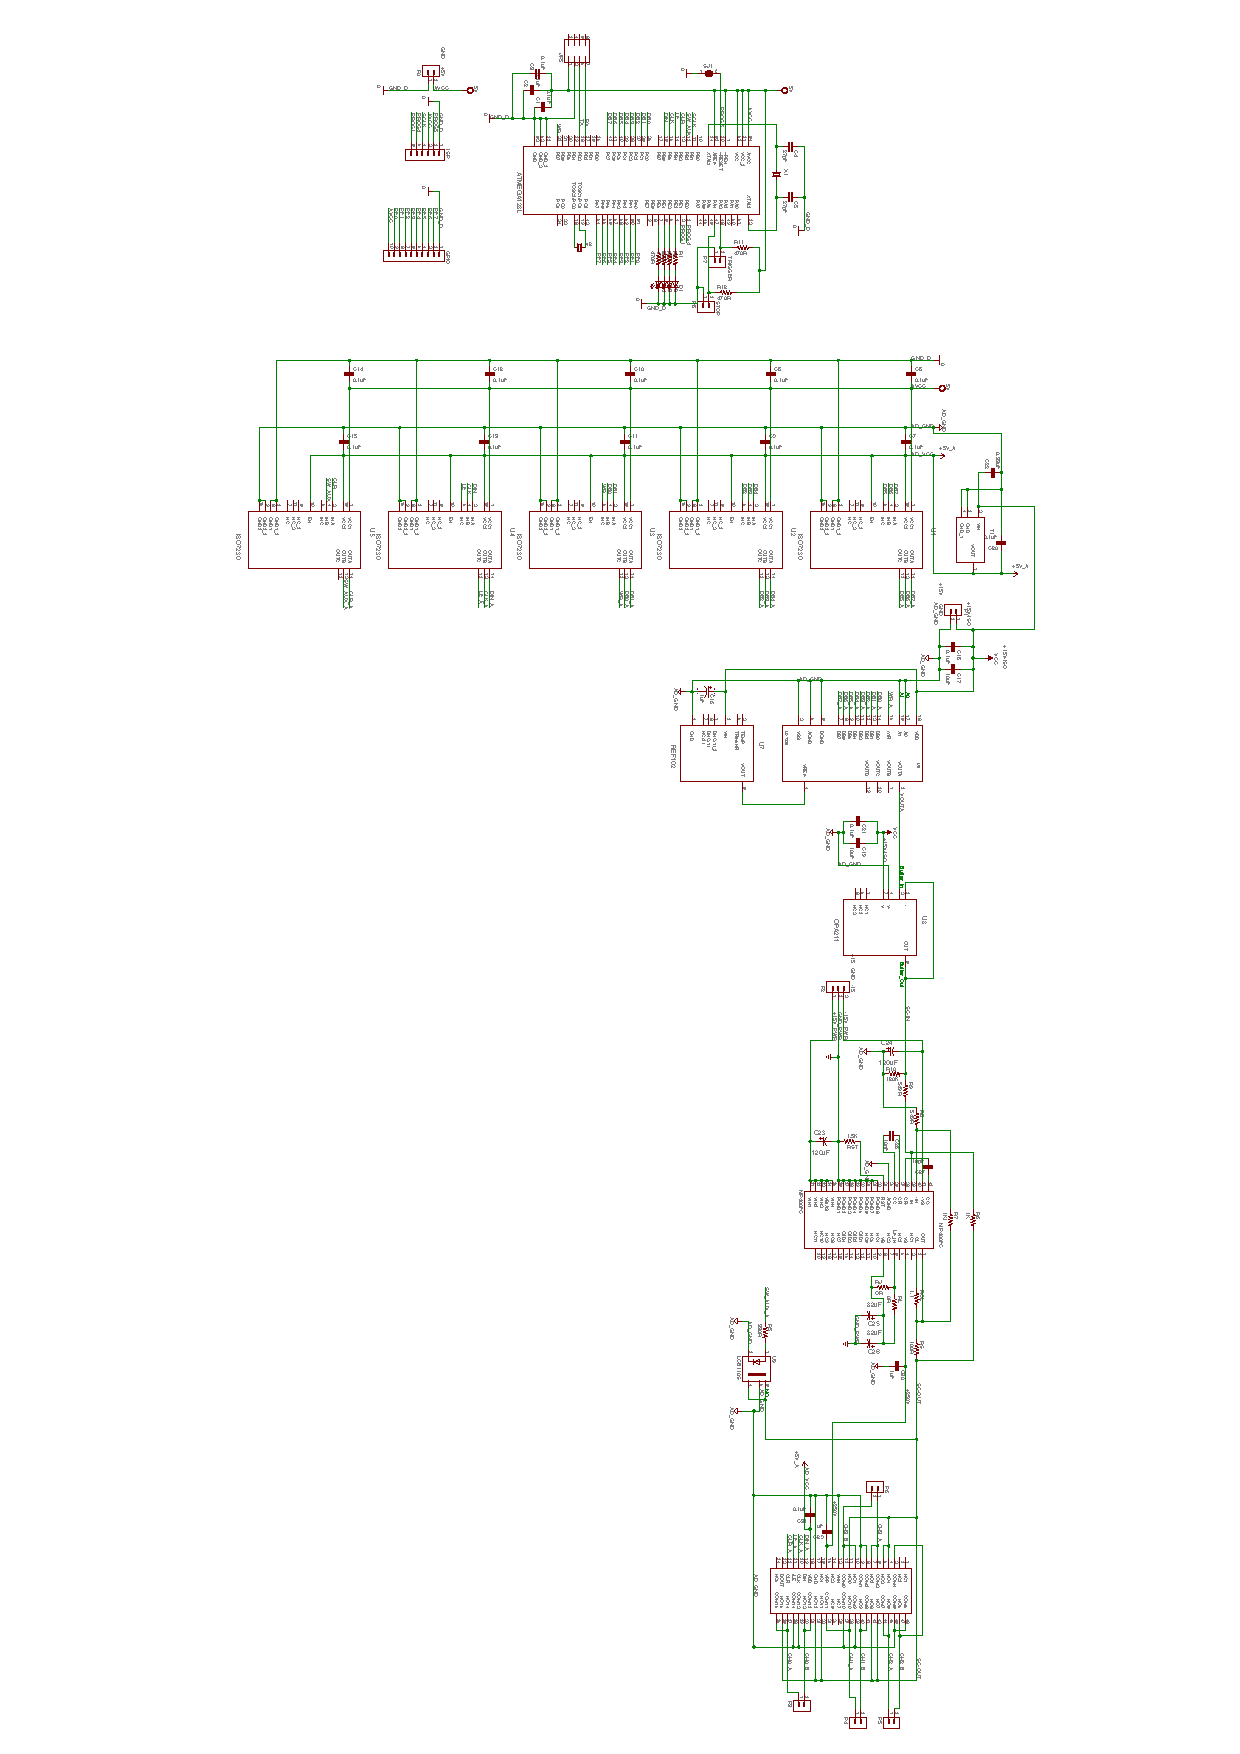
\includepdf[page={1},scale=1.0]{4CH_V2_rotado}\label{esquematico_control}

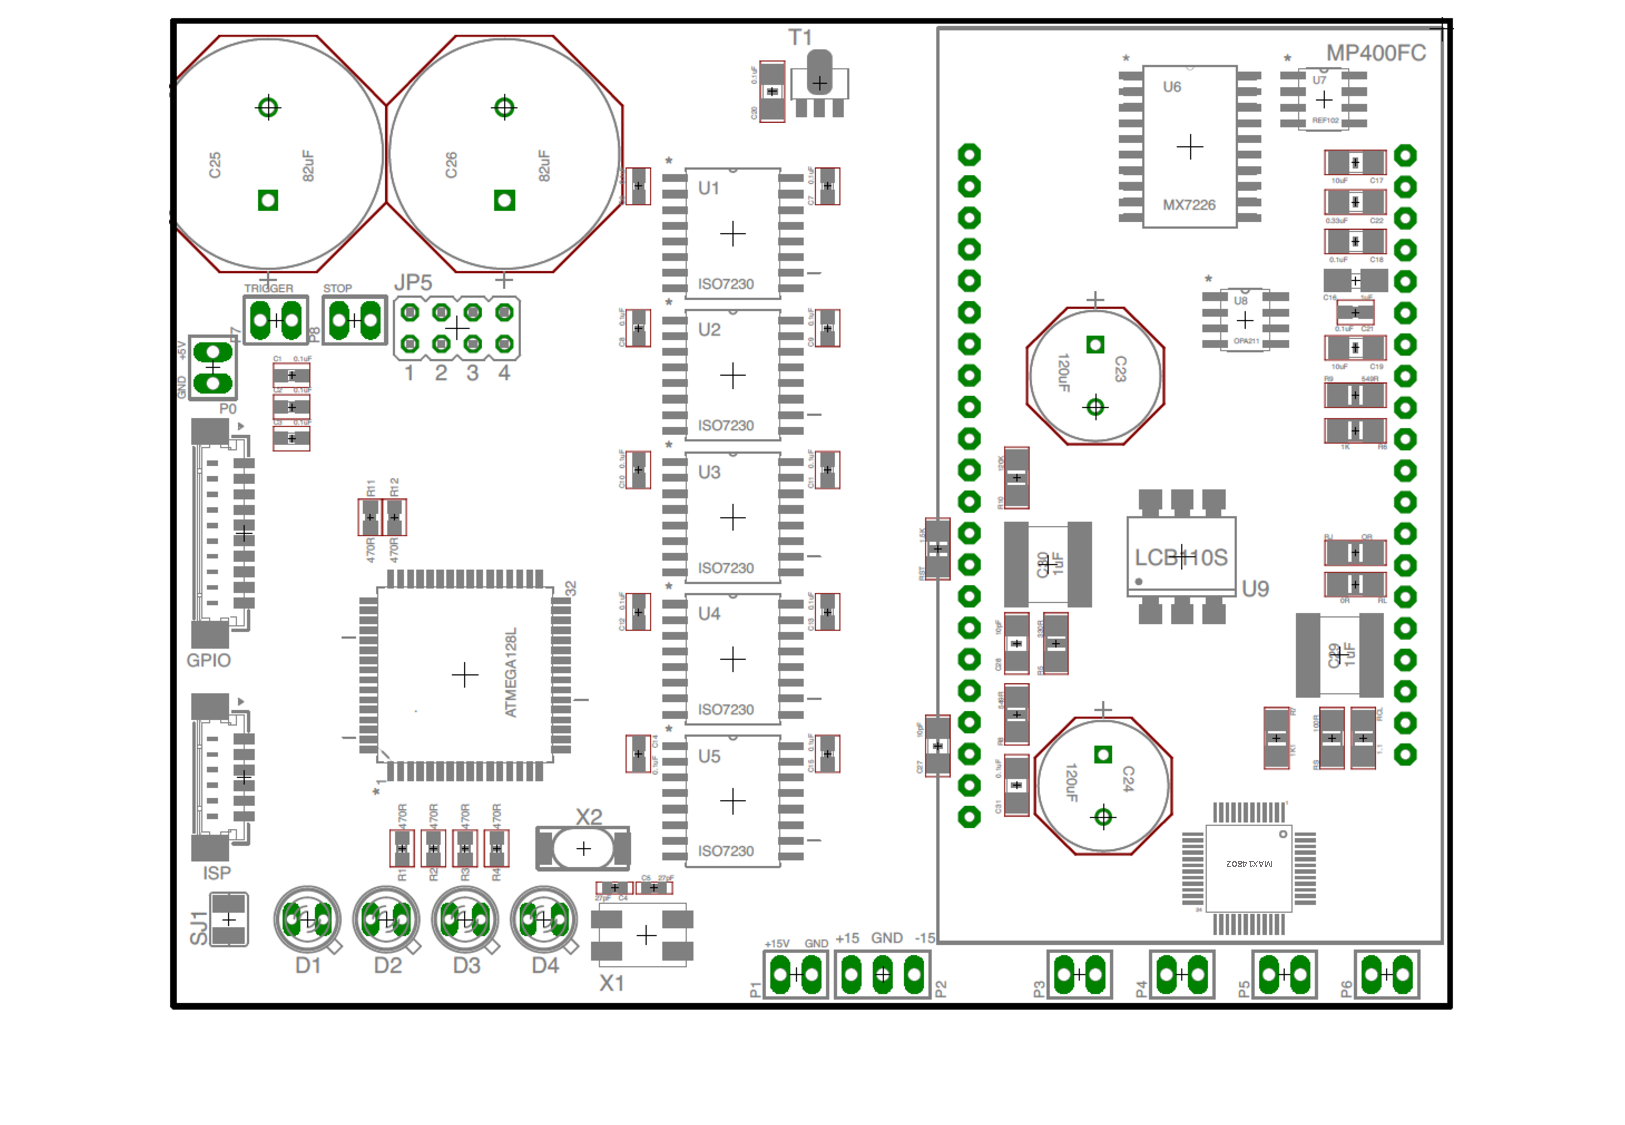
\includepdf[page={1}]{4CH_BOARD}\label{placa_control}

\begin{figure}[!htb]
\centering
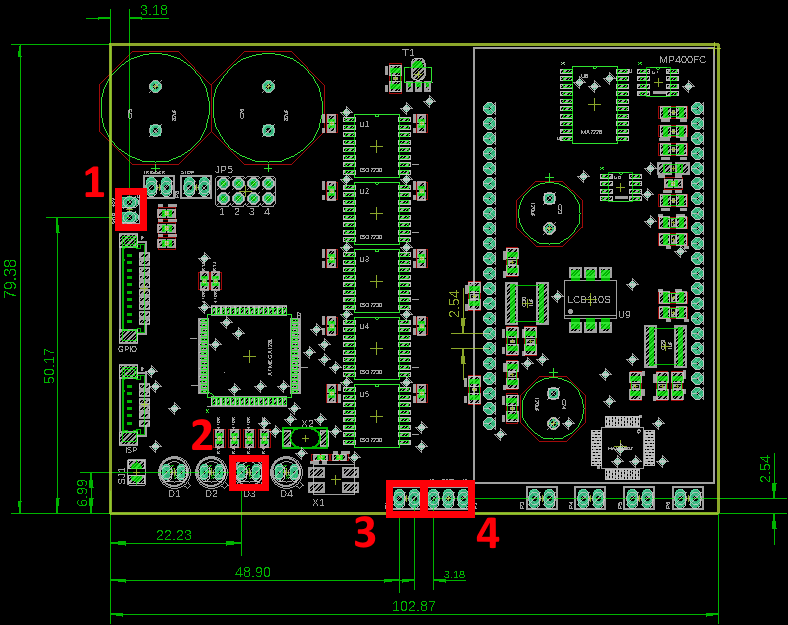
\includegraphics[scale=1.0]{pcb_control_layout}
  \caption{Distribución de componentes en el anverso de la tarjeta de circuito impreso de la etapa de control del mini TEREFES. En color rojo se indican los conectores explicados en la figura \ref{fig:montaje_alineado}}\label{fig:pcb_control_layout}
\end{figure}


%------------------ANEXO II--------------------
\chapter{Anexo II: Documentación de la etapa de potencia}\label{anexo2}
\newpage

\begin{figure}[!htb]
\centering
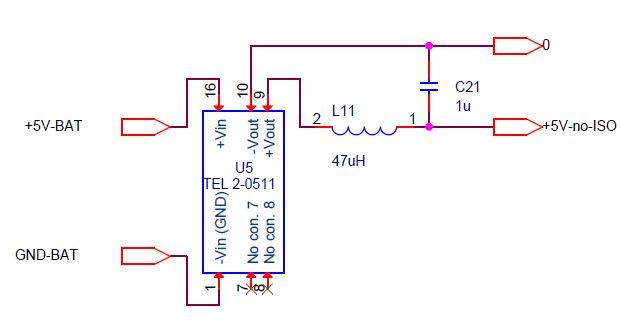
\includegraphics[scale=0.7]{fuente5vdc_esquematico}
  \caption{Fuente de $5VDC$.}\label{fig:fuente5vdc_esquematico}
\end{figure}


\begin{figure}[!htb]
\centering
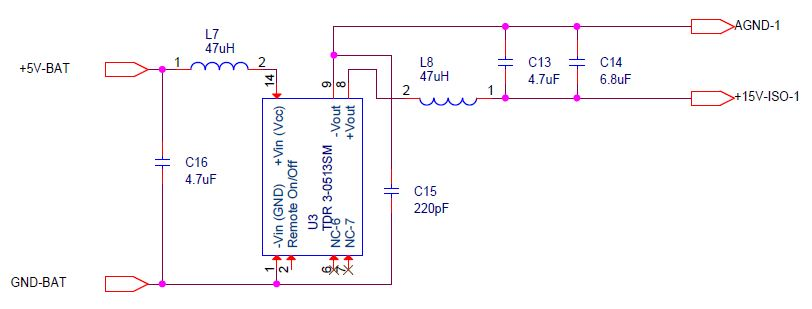
\includegraphics[scale=0.7]{fuente15vdc_esquematico}
  \caption{Fuente de $15VDC$.}\label{fig:fuente15vdc_esquematico}
\end{figure}


\begin{figure}[!htb]
\centering
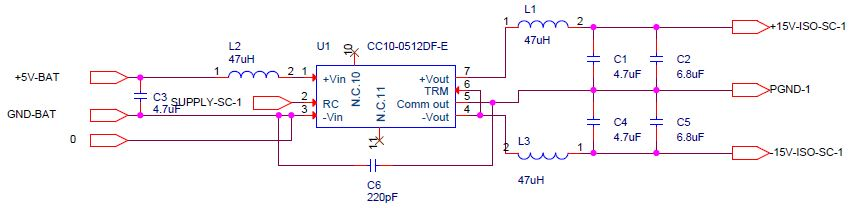
\includegraphics[scale=0.7]{fuente+-15vdc_esquematico}
  \caption{Fuente de $\pm15VDC$.}\label{fig:fuente+-15vdc_esquematico}
\end{figure}

\begin{figure}[!htb]
\centering
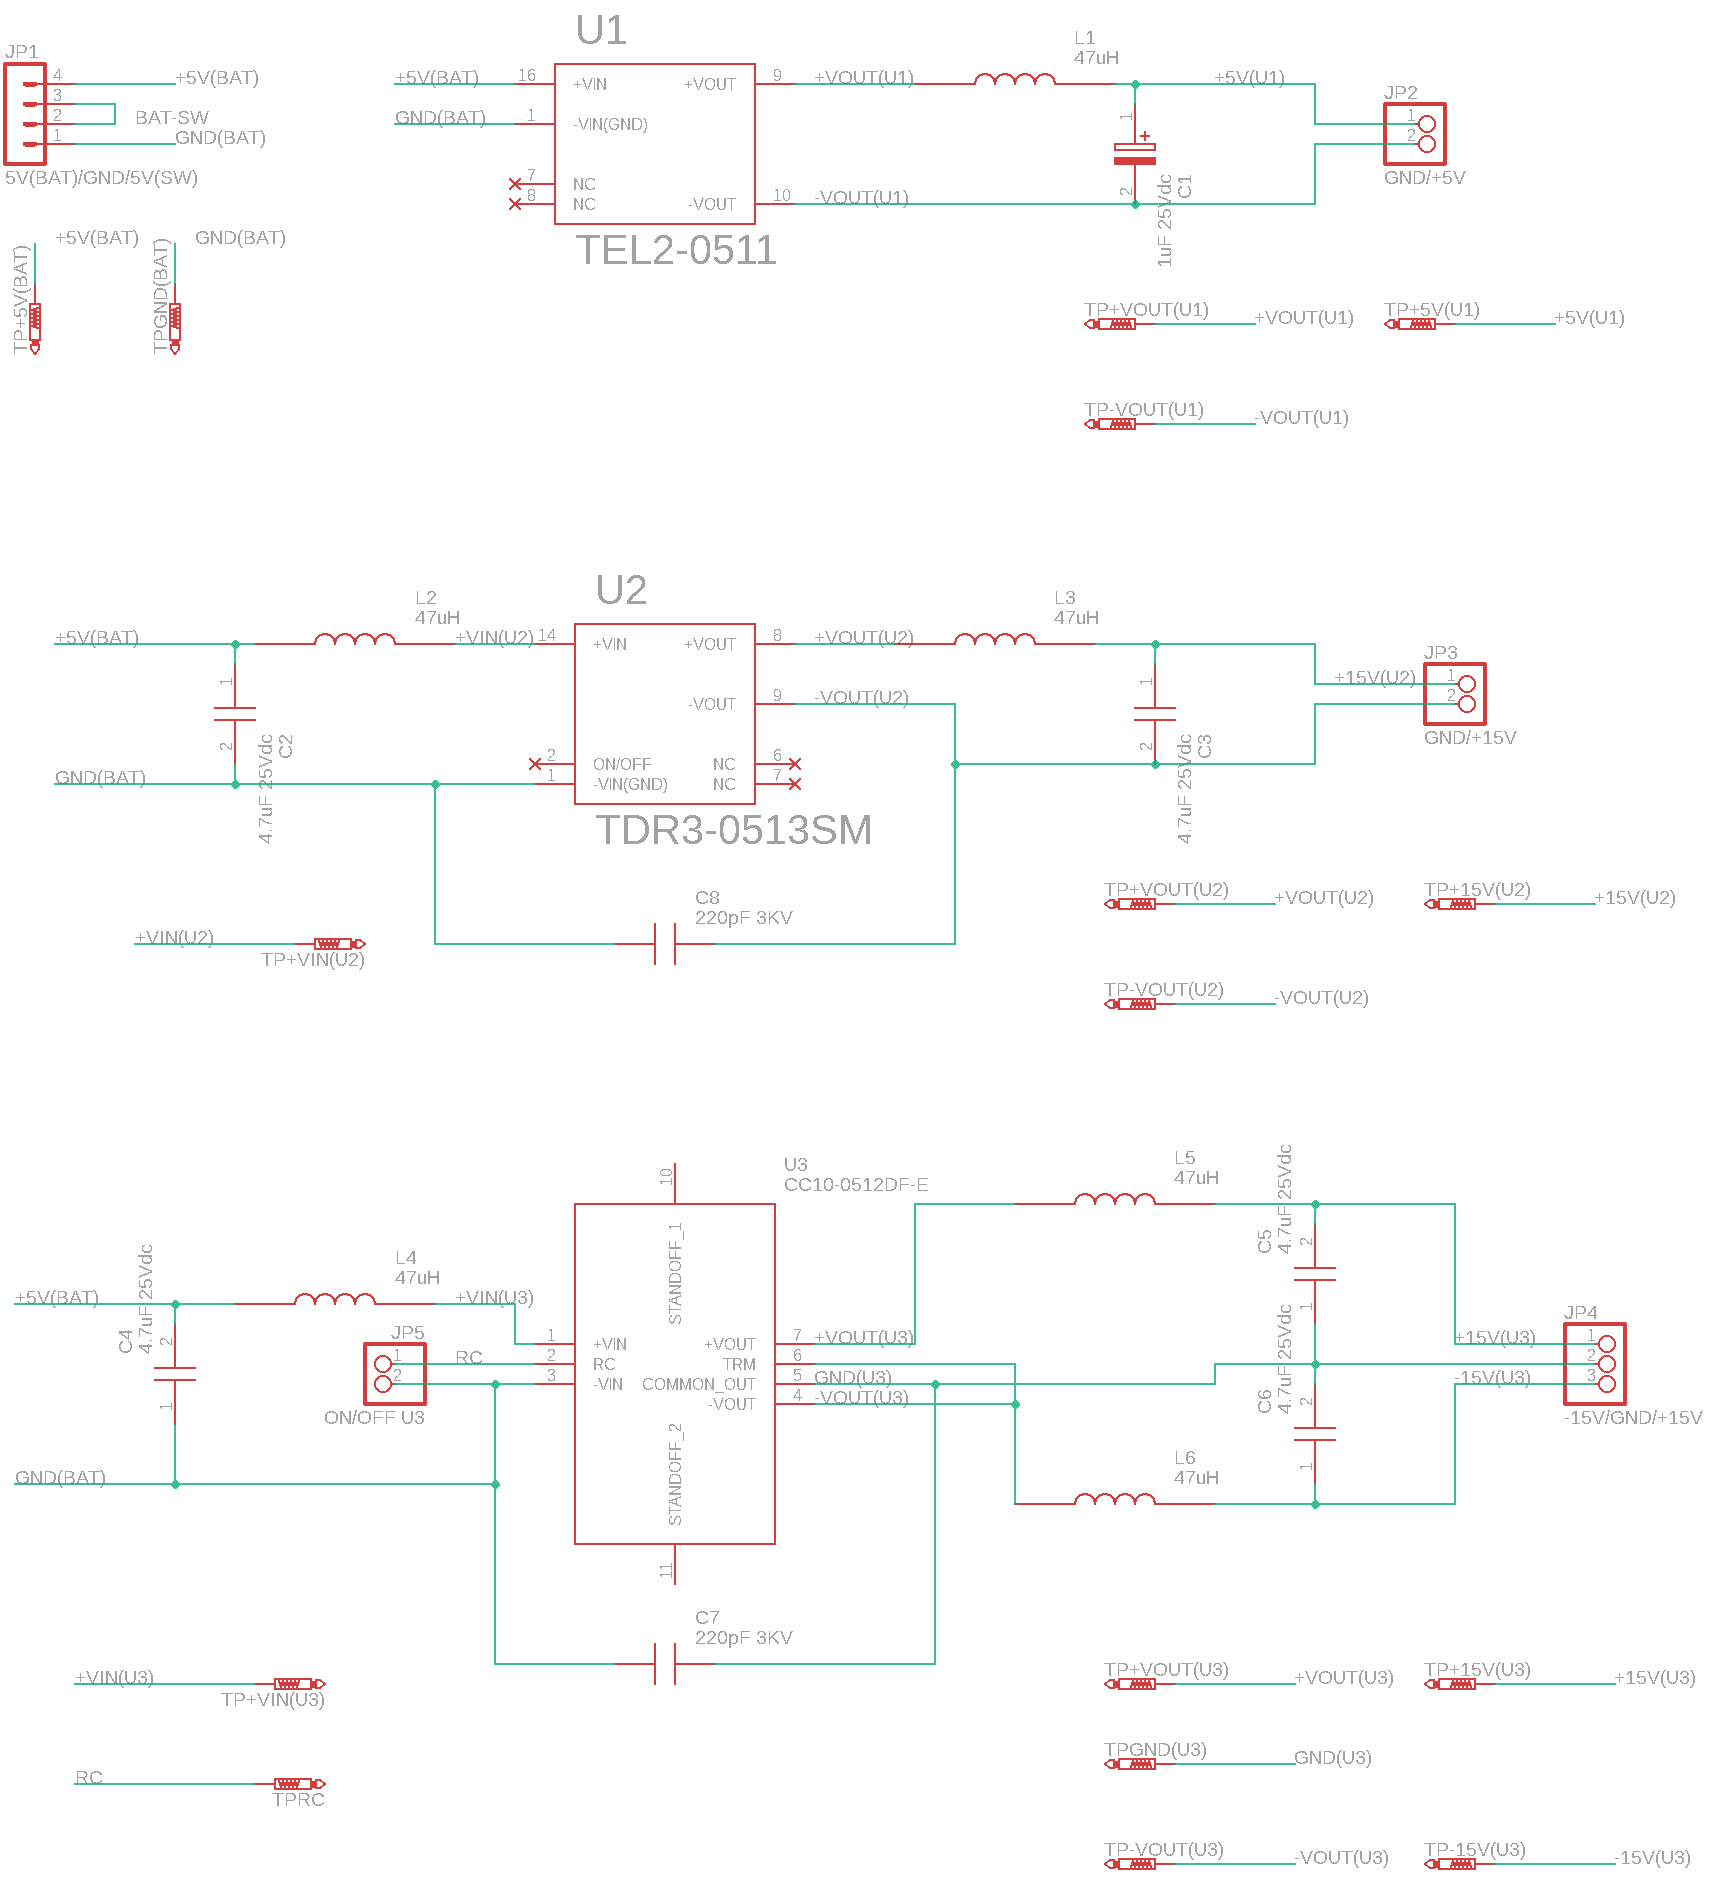
\includegraphics[scale=0.8]{pcb_potencia_esquematico}
  \caption{Esquemático de la etapa de potencia del mini TEREFES.}\label{fig:pcb_potencia_esquematico}
\end{figure}

\begin{figure}[!htb]
\centering
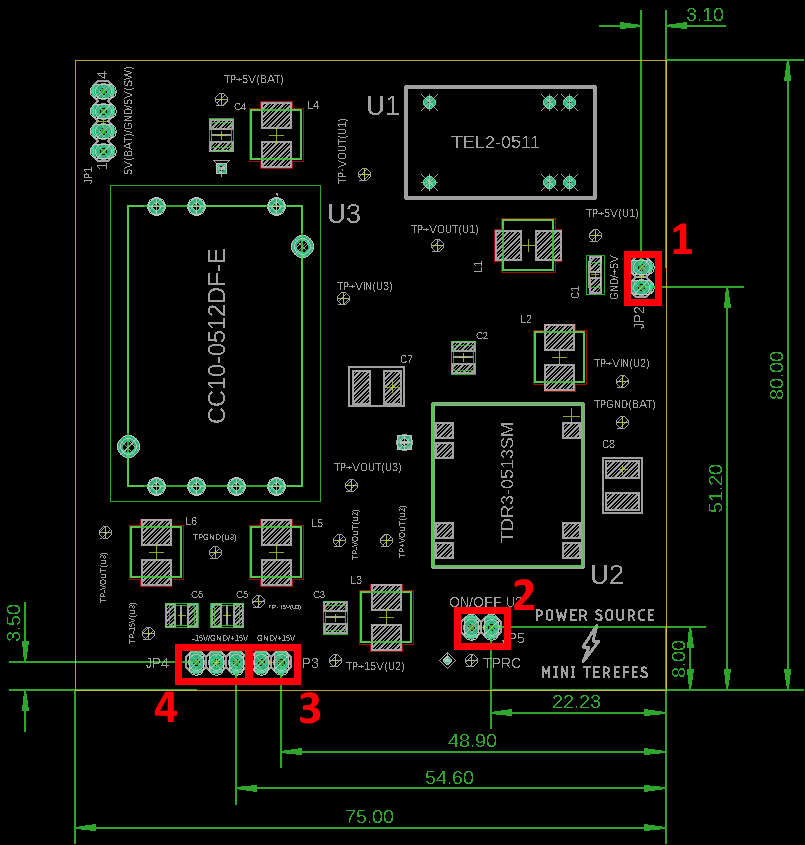
\includegraphics[scale=1.0]{pcb_potencia_layout}
  \caption{Distribución de componentes en el anverso de la tarjeta de circuito impreso de la etapa de potencia del mini TEREFES. En color rojo se indican los conectores explicados en la figura \ref{fig:montaje_alineado}}\label{fig:pcb_potencia_layout}
\end{figure}

\begin{figure}[!htb]
\centering
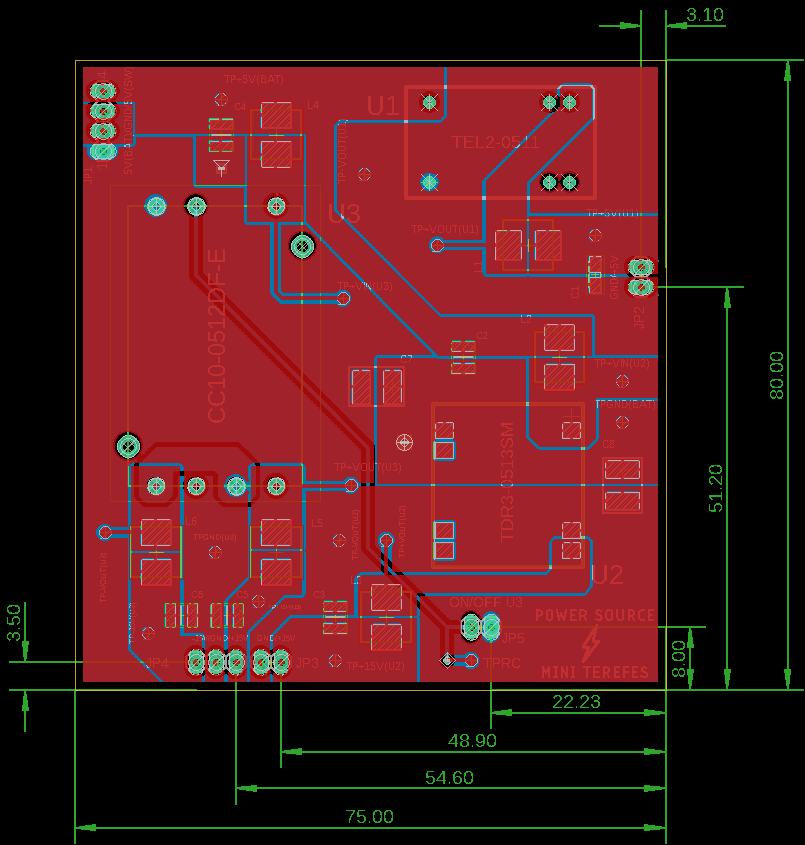
\includegraphics[scale=1.0]{pcb_potencia_top}
  \caption{Capa superior de la placa de potencia del mini TEREFES.}\label{fig:pcb_potencia_top}
\end{figure}

\begin{figure}[!htb]
\centering
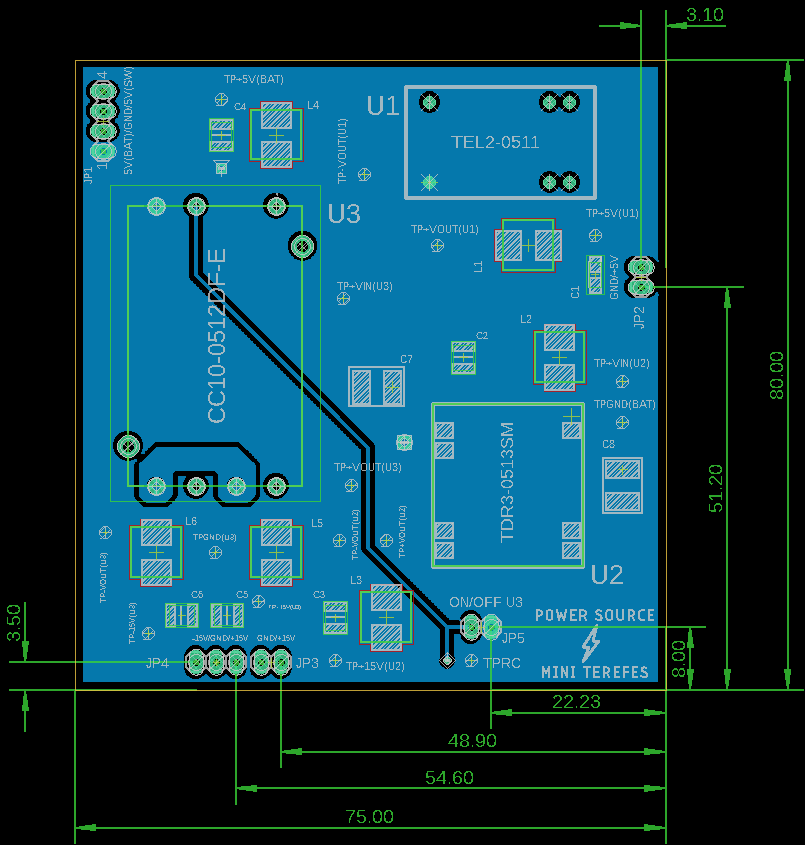
\includegraphics[scale=1.0]{pcb_potencia_bottom}
  \caption{Capa inferior de la placa de potencia del mini TEREFES.}\label{fig:pcb_potencia_bottom}
\end{figure}

\begin{figure}[!htb]
\centering
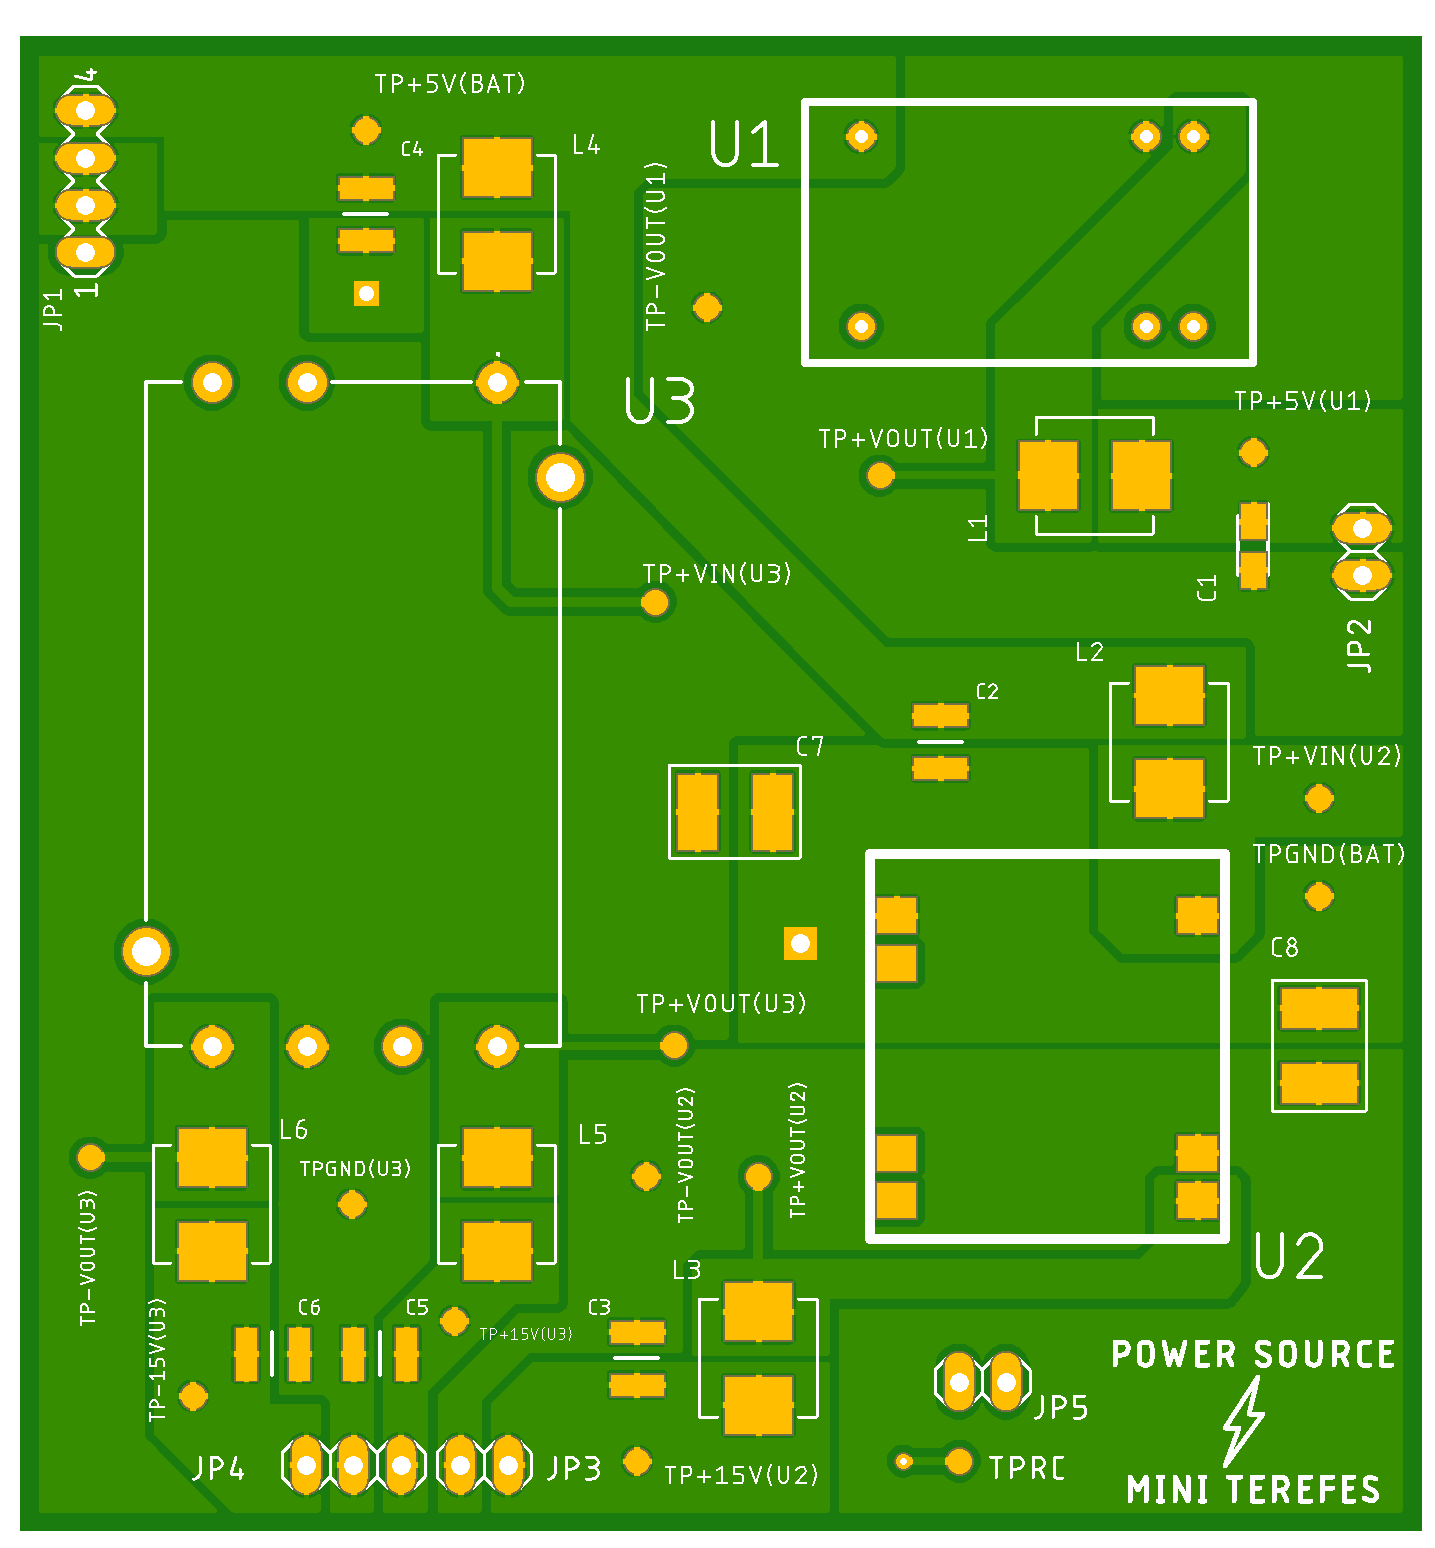
\includegraphics[scale=0.25]{pcb_potencia_modelo}
  \caption{Modelo de la placa de potencia del mini TEREFES.}\label{fig:pcb_potencia_modelo}
\end{figure}